\documentclass[review,12pt]{elsarticle}
\usepackage{booktabs,tabularx,array,longtable,graphicx,float,pdflscape,url,hyperref}
\hypersetup{hidelinks}
\usepackage[T1]{fontenc}
\usepackage[utf8]{inputenc}
\setlength{\emergencystretch}{3em}
\renewcommand{\thesection}{S\arabic{section}}
\renewcommand{\thefigure}{S\arabic{figure}}
\renewcommand{\thetable}{S\arabic{table}}
\begin{document}
\begin{frontmatter}
\title{Supplementary information for the OpenDC-LCA transferability audit}
\author[uark,hfa]{Braden Stevens}
\author[uark,hfa]{Pengjiang Xiang}
\author[ornl]{Yimin Chen}
\author[uark]{Darin Nutter}
\author[uark]{Han Hu}
\address[uark]{Department of Mechanical Engineering, University of Arkansas, Fayetteville, AR 72701, U.S.}
\address[ornl]{Building Technologies Research and Integration Center, Oak Ridge National Laboratory, Oak Ridge, TN 37830, U.S.}
\address[hfa]{Harrison French \& Associates Ltd., Bentonville, AR 72712, U.S.}
\end{frontmatter}

This supplement documents secondary analyses, software fixtures, and reproducibility details. It must be interpreted with the evidence classes and claim limits in the main manuscript.

\section{Evidence inventory and provenance}
The source registry records each provider-native file, version, access URL, declared license or redistribution constraint, local filename, and SHA-256 checksum. Files with uncertain redistribution rights remain under \texttt{private-data/} and are excluded from Git. Derived tables are written to both \texttt{paper/tables/} and a results directory.

The checksum ledger contains 42 provider files, including all nine historical eGRID downloads. The Applied Energy execution metadata records the files that enter its numerical results, all directly imported analysis modules, the Python runtime, Git commit and dirty-state digest, fixed seeds and iterations, and hashes for every generated table and figure. A provider catalog is not treated as an execution manifest.

Provider fields used in the analyses are:

\begin{itemize}
\item Microsoft/WSP: normalized GHG, primary-energy, and blue-water contribution
tables; detailed GaBi electricity endpoints; pedigree assessment.

\item eGRID: state and U.S. generation, CO2, CH4, N2O, and reported CO2e rates.
\item Federal LCA Commons: openLCA process exchanges, product-system links, unit
groups, and IPCC AR5-100 characterization factors.

\item Boavizta: product category, manufacturer, product name, report date,
lifetime, total GWP, and manufacturing share.

\item ÖKOBAUDAT: UUID, product, geography, declared unit, modules A1-A3, GWP,
nonrenewable primary energy, and freshwater.

\end{itemize}

USLCI, GLAD hydrogen, and USGS records are registered and exchange-tested but do not enter a reported cooling LCIA total.

\section{Reproducibility table map}
{\small
\setlength{\tabcolsep}{4pt}
\begin{longtable}{>{\raggedright\arraybackslash}p{0.38\textwidth}>{\raggedright\arraybackslash}p{0.27\textwidth}>{\raggedright\arraybackslash}p{0.27\textwidth}}
\caption{Supplementary result map}\\
\toprule
File & Content & Evidence interpretation \\
\midrule
\endfirsthead
\caption[]{Supplementary result map (continued)}\\
\toprule
File & Content & Evidence interpretation \\
\midrule
\endhead
\midrule
\multicolumn{3}{r}{Continued on next page}\\
\endfoot
\bottomrule
\endlastfoot
\path{table1_microsoft_reproduction_audit.csv} & 24 released totals and reconstruction error & Arithmetic consistency only \\
\path{table2_grid_reductions_vs_air.csv} & Relative reductions from the released model & Reconstructed released result \\
\path{table6_state_rebased_ghg.csv} & 2023 state screening outputs & Boundary-mismatched numerical transfer \\
\path{table8_crossover_thresholds.csv} & Pairwise crossover values & Conditional numerical landmarks \\
\path{table9_boavizta_server_records.csv} & 48 included public product records & Heterogeneous secondary evidence \\
\path{table14_egrid_historical_state_factors.csv} & 459 harmonized state-year rates & Direct generation-rate scenarios \\
\path{table15_egrid_historical_national_factors.csv} & Harmonized and provider U.S. series & Historical trend and scope audit \\
\path{table21_anchor_extrapolation_diagnostic.csv} & Within/below/above anchor counts & Transformation-validity diagnostic \\
\path{table22_boundary_mismatch_stress.csv} & Additive allowance cases & Sensitivity, not an upstream estimate \\
\path{table23_joint_assumption_stress.csv} & Seeded stress frequencies & Not probability or confidence \\
\path{table24_functional_unit_sensitivity.csv} & Impact-per-service break-even correction & Measurement-resolution target \\
\path{table25_priority_index_sensitivity.csv} & Rank stability across index weights & Heuristic diagnostic \\
\path{table26_stress_structure_sensitivity.csv} & Assumption-block and dependence designs & Design sensitivity, not empirical probability \\
\path{table28_lifecycle_electricity_factors.csv} & 71 ordinary at-user consumption systems & Partial provider-linked LCI with documented cutoffs \\
\path{table29_standardized_rank_robustness.csv} & Exact equal-width reversal bounds & Deterministic uncertainty sets \\
\path{table30_released_endpoint_method_audit.csv} & Article/workbook method conflict & Blocks a common-method cooling claim \\
\path{table31_implied_electricity_response.csv} & Slopes implied by released endpoints & Diagnostic response, not measured demand \\
\path{table32_national_lifecycle_cutoffs.csv} & National unlinked inputs & Omitted-upstream audit \\
\path{table33_residual_electricity_factors.csv} & Separate residual-consumption systems & Market-based accounting sensitivity \\
\path{table34_boavizta_server_inclusion.csv} & All 55 candidates and reasons & Transparent inclusion/exclusion flow \\
\end{longtable}
}

\section{Released lifecycle results}
The 24-cell reconstruction includes GHG, primary energy, and blue water. The main manuscript focuses on GHG because the historical eGRID extension supplies gas-specific air-emission data, not lifecycle primary-energy or electricity-mediated water inventories. The other indicators inherit the released functional unit, boundary, allocation, performance, and electricity cases and were not re-based with eGRID.

\section{Endpoint and crossover diagnostics}
The article identifies AR5 GWP100, but the detailed public workbook contains the two numeric electricity endpoints in cells labelled GTP100, while its corresponding GWP100 cells are blank. Direct worksheet-XML parsing verifies that comparative use-phase formulas \texttt{Comparative results 0\% RE!D118} and \texttt{Comparative results 100\% RE!D122} point to those blank F29 cells. This unresolved method identity prevents treatment of the cooling screen as a common-method LCA.

\begin{figure}[H]
\centering
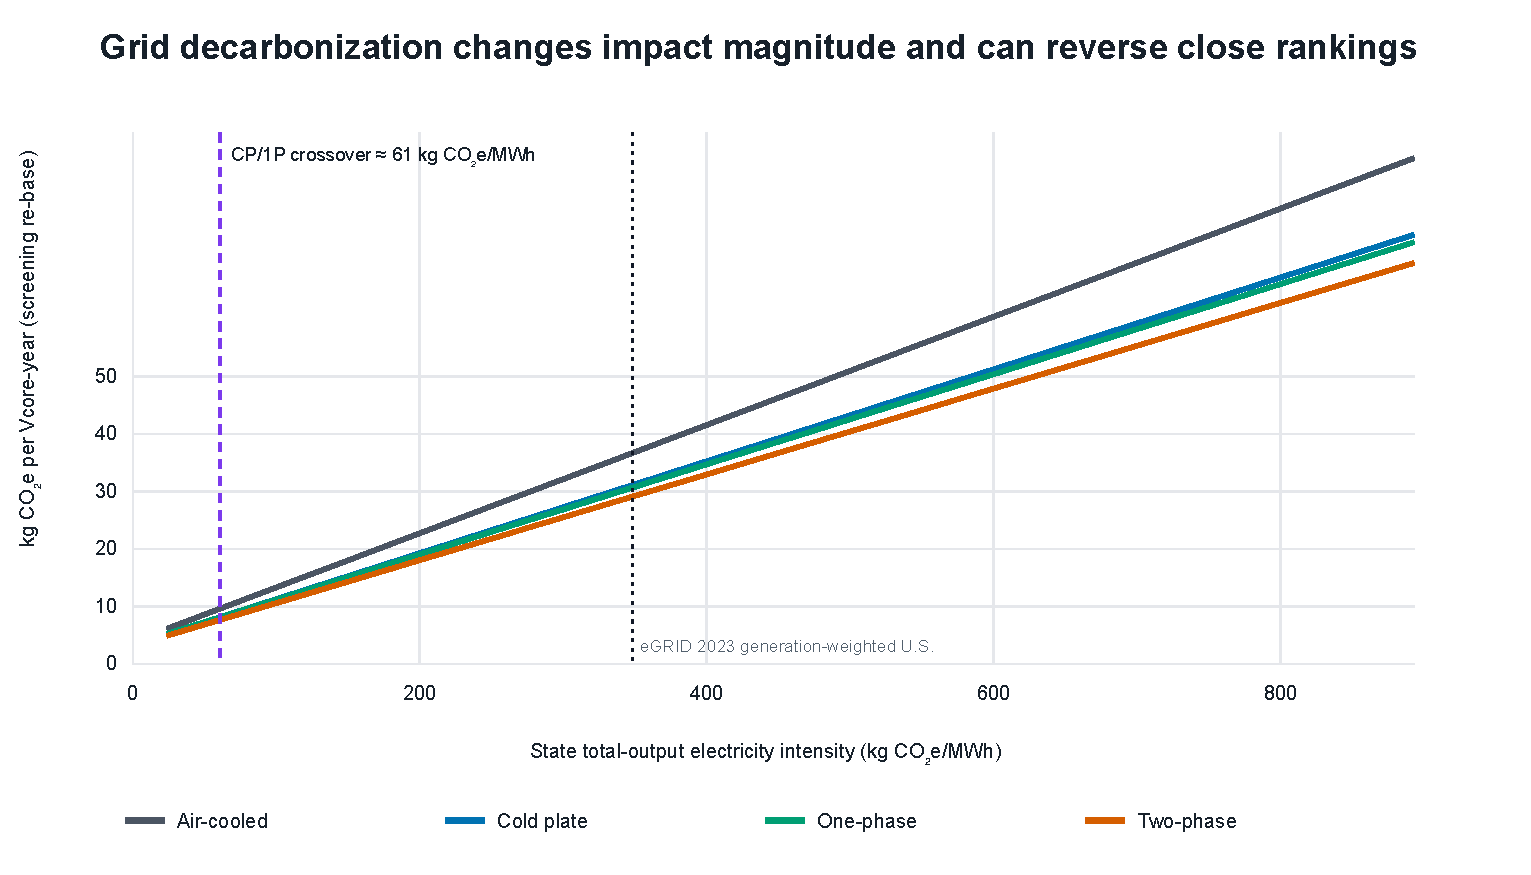
\includegraphics[width=0.96\linewidth]{figures/figure2_grid_crossover.pdf}
\caption{Screening totals transferred across 2023 eGRID state/DC rates. The vertical line is the cold-plate/single-phase numerical crossover. The x-axis is an electricity-intensity index across incompatible lifecycle boundaries, not a background-process substitution.}
\end{figure}

The two-phase numerical line has no crossover with cold plate or single-phase inside the 2023 state-rate range under the fixed released foreground. This is conditional on server performance, fluid, equipment quantity, lifetime, and the numerical transfer model.

\section{Electricity-system calculation}
The 2023 ordinary consumption systems comprise 60 balancing authorities, 10 FERC regions, and the national system. The national partial linked-system result is 422.931 kg CO2e/MWh, with 369.848 from named generation processes and 53.084 from other linked processes. The matched residual-consumption result is 455.350 kg CO2e/MWh and is kept separate.

The national ordinary system solves 582 processes and 1,174 provider links in five fixed-point iterations. It retains 287 unlinked technosphere inputs across 47 processes as explicit cutoffs. Provider scope also omits transmission/distribution infrastructure and some generation infrastructure. The results are partial-scope screening factors, not complete electricity lifecycle benchmarks. The custom solver has an analytic unit-conversion, provider-scaling, elementary-flow-sign, and cutoff test, but independent reproduction in openLCA or Brightway remains a submission action.

\section{Robustness analyses}
\begin{figure}[H]
\centering
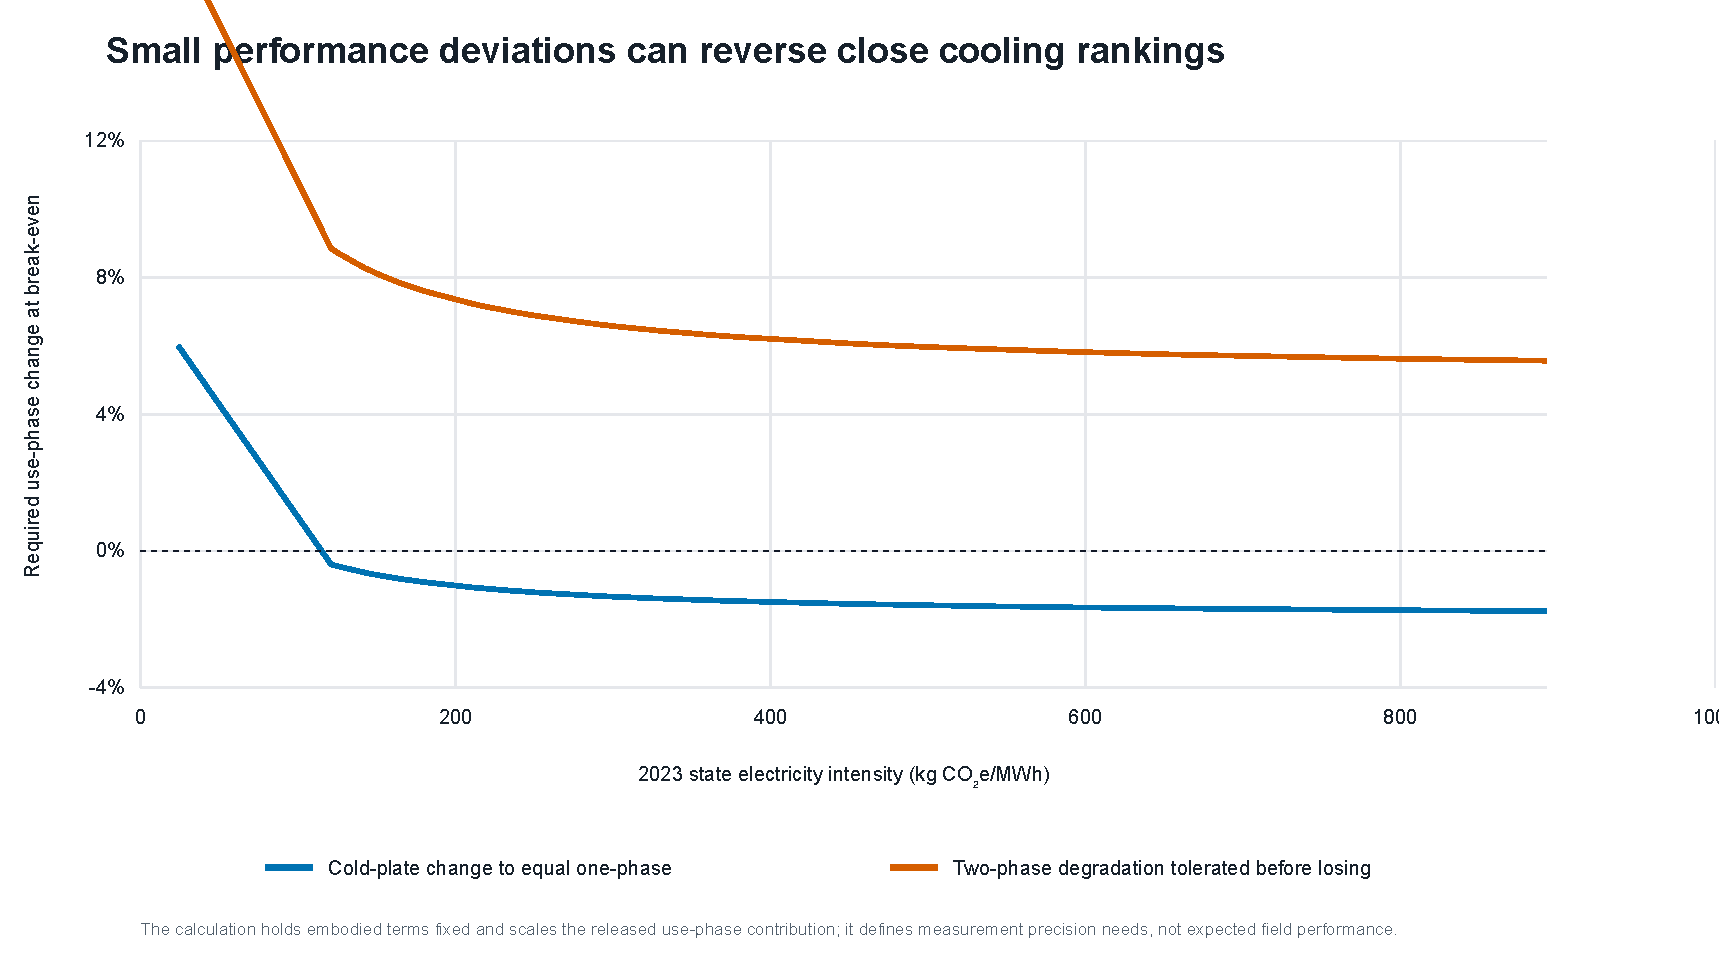
\includegraphics[width=0.96\linewidth]{figures/figure7_performance_robustness.pdf}
\caption{One-at-a-time use-phase change required to alter close rankings across 2023 state rates. These thresholds are experimental discrimination targets, not uncertainty intervals.}
\end{figure}

At equal relative half-widths, the national first-rank screen reverses at 2.99\% for technology-specific use phase, 22.15\% for embodied burden, 2.64\% for service equivalence, and 1.32\% when all four blocks vary. The shared grid-only set does not reverse the order through 99.999\%. These are exact set-based certificates around the numerical screen, not physical validation.

The earlier triangular design assigned embodied burden a half-width ten times the use-phase and service widths. Within that declared wide design, embodied-only variation gave a 63.36\% two-phase first-rank frequency, compared with 79.52\% for use only, 73.90\% for service only, and 100\% for grid only. The frequencies describe that stress design, not empirical uncertainty. \texttt{table27\_stress\_convergence.csv} records nested 5,000-, 20,000-, and 80,000-draw checks and numerical Monte Carlo standard errors.

\section{Server-product evidence}
\begin{figure}[H]
\centering
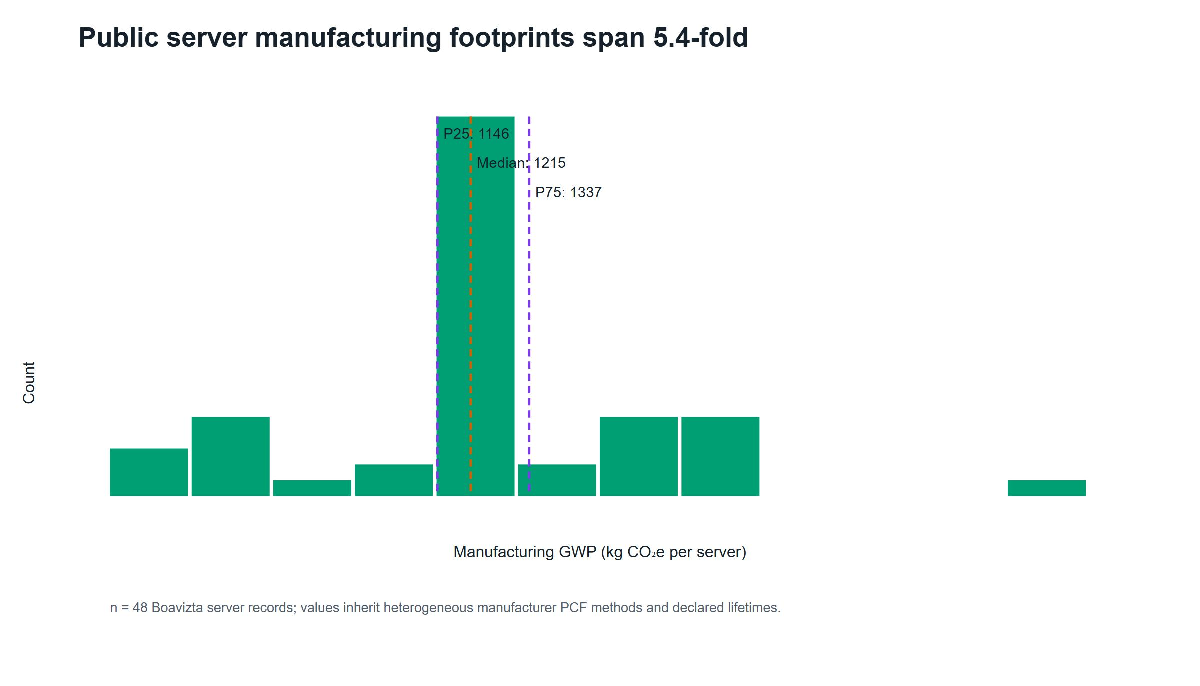
\includegraphics[width=0.96\linewidth]{figures/figure4_server_epd_distribution.pdf}
\caption{Distribution of manufacturing GHG across 48 included Boavizta server records. The records inherit heterogeneous product rules, hardware configurations, lifetimes, and source methods.}
\end{figure}

All 55 \texttt{Datacenter/Server} candidates appear in Table 34. Forty-eight contain total GWP, manufacturing share, and positive lifetime. Seven Lenovo records are excluded because manufacturing share is blank. The common-scaling stress uses included annualized dispersion but is not a product-substitution model. Decision use requires architecture-specific server count, configuration, useful computation, and lifetime under harmonized product rules.

\section{Construction-material screening}
\begin{figure}[H]
\centering
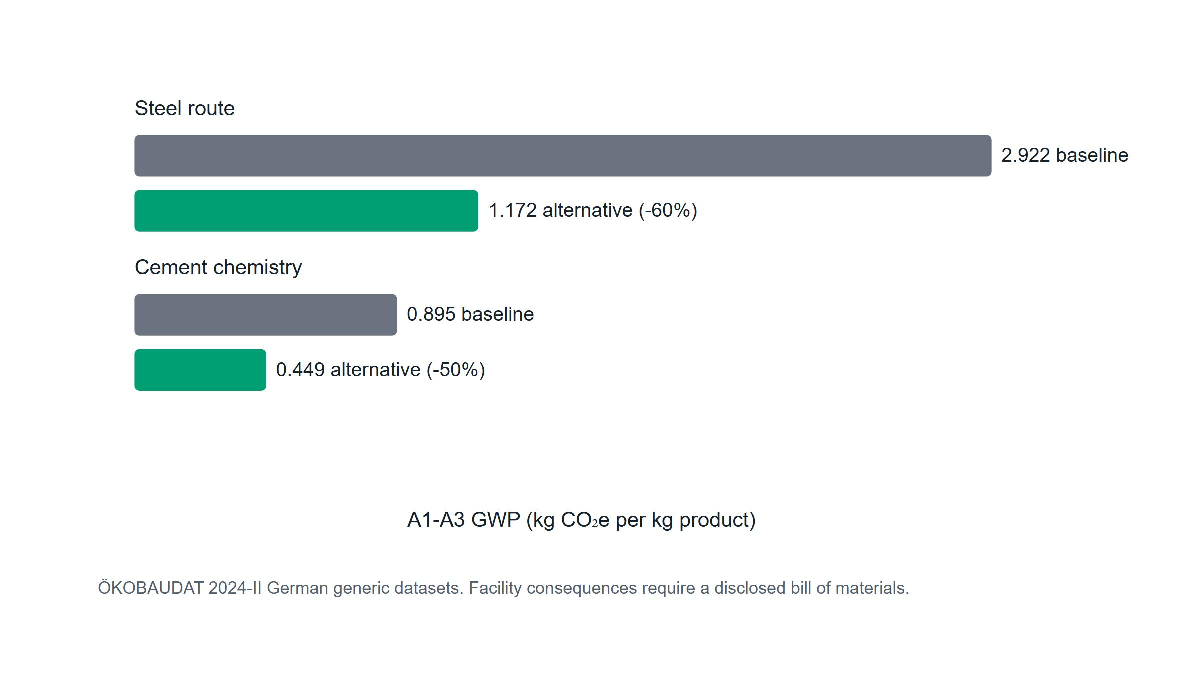
\includegraphics[width=0.96\linewidth]{figures/figure5_material_levers.pdf}
\caption{Selected matched ÖKOBAUDAT A1-A3 GHG factors. The comparison identifies per-kilogram procurement leverage and is not propagated to a data-center total.}
\end{figure}

The selected records are German generic datasets. A facility analysis requires architecture-specific quantities, material grade and supplier, fabrication, transport, replacement, and end-of-life alignment.

\section{Climate and performance-map fixtures}
The Fayetteville TMY file contains 8,760 hourly weather records. It is paired with a synthetic performance surface to test schema and unit validation, bounded bilinear interpolation, uncovered-domain rejection, cooling-only partial-PUE integration with one constant grid factor, and interface consistency.

\begin{figure}[H]
\centering
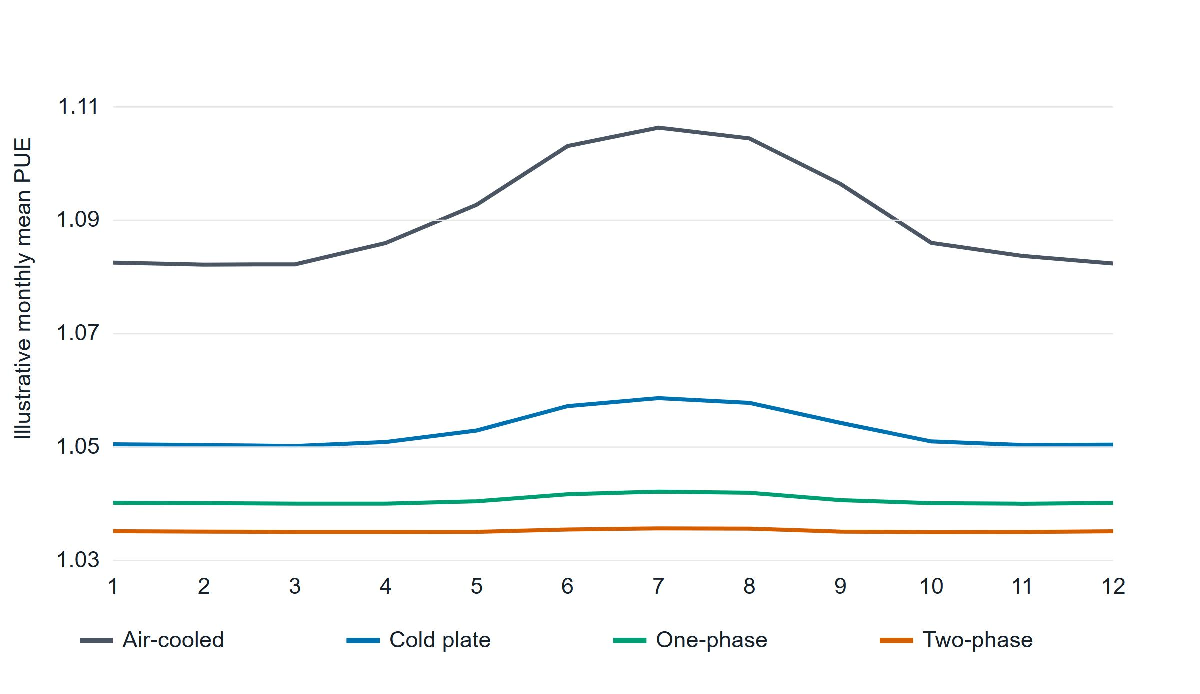
\includegraphics[width=0.96\linewidth]{figures/figure2_monthly_climate_pue.pdf}
\caption{Monthly cooling-only partial PUE from the Fayetteville weather and declared illustrative performance surface. This is a software fixture, not empirical evidence for a cooling technology.}
\end{figure}

\begin{figure}[H]
\centering
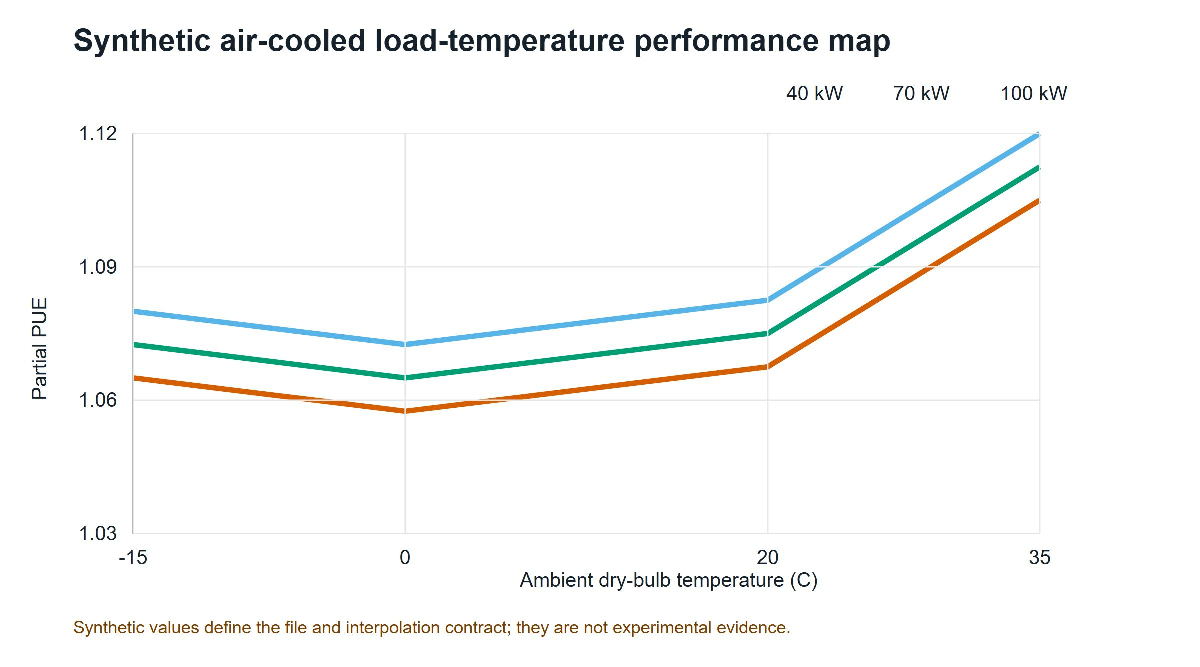
\includegraphics[width=0.96\linewidth]{figures/figure5_synthetic_performance_surface.pdf}
\caption{Synthetic load-temperature cooling surface used to verify bounded interpolation. No comparative assertion is permitted from this fixture.}
\end{figure}

Wet-bulb temperature is validated in the input schema but is not an interpolation coordinate. Other facility overhead is outside the partial-PUE boundary unless included in the supplied cooling-power field. Submission-grade results require architecture-specific measured power for IT-integral fans, pumps, coolant distribution, heat rejection, controls, and onsite water over a common load-weather domain, plus an energy-balance residual.

\section{Data-priority diagnostic}
The base index multiplies mean released GHG contribution by normalized pedigree weakness. Alternative exponents show that use phase is usually, but not always, first; storage remains in the top tier. This is not formal value of information. Formal analysis would require empirical distributions and correlations, the probability and consequence of a wrong choice, measurement cost and precision, a decision threshold, stakeholder utility, and posterior updating.

\section{Reliability and interoperability}
The package supports discrete replacement, linearized replacement, Weibull renewal expectation, and optional Arrhenius acceleration. These functions do not supply architecture-specific reliability without failure, maintenance, duty-cycle, temperature, censoring, and downtime records. Dependent failures, redundancy, and repair queues require an extended model.

Successful openLCA JSON-LD parsing or Brightway mapping establishes syntactic exchange only. Numerical compatibility also requires matching reference product and unit, provider and database version, geography and year, system model, allocation, cutoff, elementary-flow nomenclature, LCIA method, and foreground linkage. USLCI and GLAD archives remain future inputs rather than silent substitutes in the current cooling results.

\section{Software claim controls}
Scenario parsing rejects non-finite numeric values. Result manifests retain the field-to-source map and stable digests of source records. Public comparison requests are blocked when functional units, boundaries, electricity accounting, allocation, LCIA methods, or replacement rules differ, or when field-level lineage is missing. A custom comparative boundary requires a structured inclusion/exclusion record that must match across scenarios.

These are metadata blockers, not authentication, parameter-level uncertainty mapping, ISO conformity, or evidence that an external review occurred. Useful computation remains a manual prerequisite because the executable functional unit is presently \texttt{it\_mwh}.

\section{Reproduction commands}
From the repository root:

\begin{verbatim}
python -m pip install -e .
python scripts/run_submission_pipeline.py --skip-refresh
\end{verbatim}

Omit \texttt{--skip-refresh} to start from provider downloads. Use \texttt{--skip-documents} when document-conversion dependencies are unavailable. The pipeline runs source-manifest creation, research, integrated-evidence, and Applied Energy analyses in order, followed by tests and document builds.

A clone without \texttt{private-data/} runs the public package tests and explicitly skips the paper-reconstruction tests. Rebuilding the paper requires locally held provider files whose hashes appear in the manifest. Archive the source manifest, execution metadata, derived tables, exact Git commit, compiled main text, and supplement together.

\end{document}
